\section{Performance Evaluation}
\label{sec:perf}

In this section, we shall first detail the experimental setting of machine info, dataset and parameters; and then present the result and analysis, showing the benefit of \sys{} against state of the art approaches.

\subsection{Experimental Setting}

Experiments were run on a machine with two Intel Xeon E5C2630 2.4GHz CPUs and 64 GB of Memory, running 64 bit Windows 7 professional system.
%
We have employed a real-world dataset Sina that consists of 24 million microblogs that are associated with 43.5K users.

With respect to the parameters of \sys{}, we use the default values as mentioned in previous sections.
Particularly, in Feature Extraction, for practical reason, we employed a smaller testing dataset to obtain the proper value of $\alpha$ for extracting \textit{Interest Feature};
in User Cluster, we studied the clustering solutions with the minimum/maximum number of clusters 2 and 10;
in Behavior Modeling, a user's recent 30 days microblogs are used for short-term interest analysis and popular words of the latest 24 hours are returned by Ring as the Hot Event keywords.

\subsection{Result and Analysis}
Next, we shall report the performance of \sys{} over each component.

\stitle{Feature Extraction}
%
Fig.\ \ref{fig:fe} shows the testing results of using various $\alpha$ values.
Apparently, \sys{} results the optimal results when $\alpha$ is 0.7, upon which the interest feature extracting is performed for the overall dataset with 43.5K users and 24 million microblogs.

\begin{figure}[!htb]
\centering
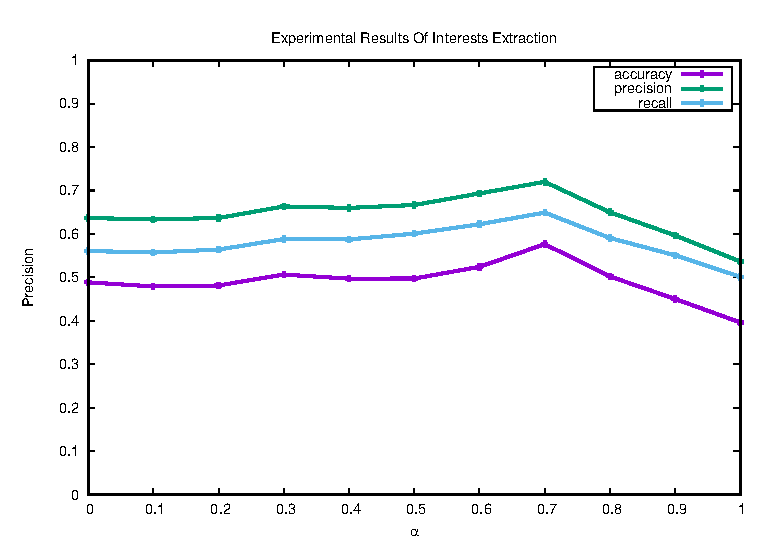
\includegraphics[width=.7\linewidth]{figures/Interests}
\caption{Testing Results with Various $\alpha$.}
\label{fig:fe}
\end{figure}


\stitle{User Clustering}
%
Fig.\ \ref{fig:uc} depicts the Silhouette Coefficient Values of multiple clustering solutions, with the cluster number from 2 to 10.
Specially, we used different testing datasets, with \textit{Data} containing the overall 43.5K users and \textit{Data1,...,5} contains 10K randomly selected users each.
Except for \textit{Data1}, solutions with 4 clusters sweep.

\begin{figure}[!htb]
\centering
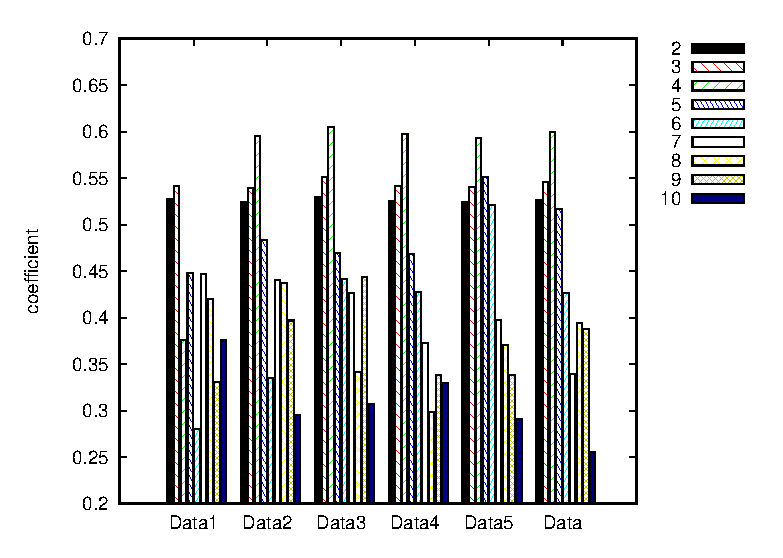
\includegraphics[width=.85\linewidth]{figures/clustering}
\caption{Silhouette Coefficient Values for Various Cluster Numbers over Different Testing Datasets.}
\label{fig:uc}
\end{figure}


\stitle{Behavior Modeling}
%
Fig.\ \ref{fig:10} shows the performance of \sys{} against state of the art approach LRC-BQ \cite{IEEEexample:conf/ijcai/ZhangLTCL13}.
We compare the metrics of precision, recall, as well as $F_1$ score.
LRC-BQ does not deal with user grouping.
Hence, we not only study the modeling effect per group (i.e., ``Group-One/Two/Three/Four'' with user clustering), but also examine \sys{} versus LRC-BQ in the case that all users are in mono group (i.e., ``All-Users'').
The results are interesting in that:
%\begin{itemize}

	\stab(1) With user clustering, \sys{} performs better than LRC-BQ in most cases.
	
	\stab(2) For \sys{}, having user clustering is better than the alternative mono group. Ditto for LRC-BQ.
%\end{itemize}



\begin{figure*}
  \centering
  \subfigure[Precision]{
    \label{fig:10-a}
    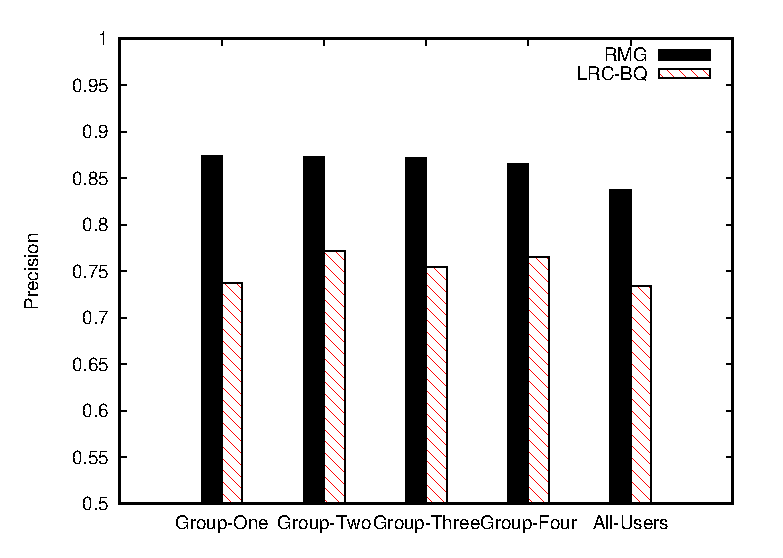
\includegraphics[width=0.32\textwidth]{figures/precision.eps}}
  %\hspace{1in}
  \subfigure[Recall]{
    \label{fig:10-b}
    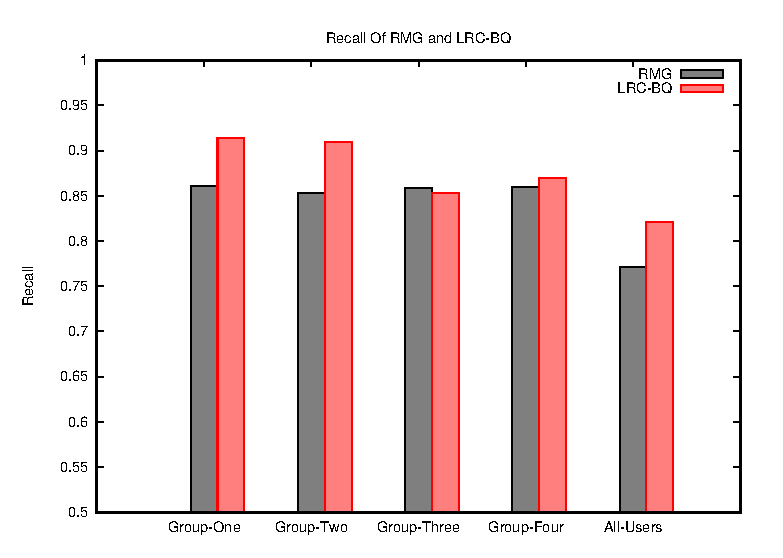
\includegraphics[width=0.32\textwidth]{figures/recall.eps}}
  %\hspace{1in}
  \subfigure[$F_1$ Score]{
    \label{fig:10-c}
    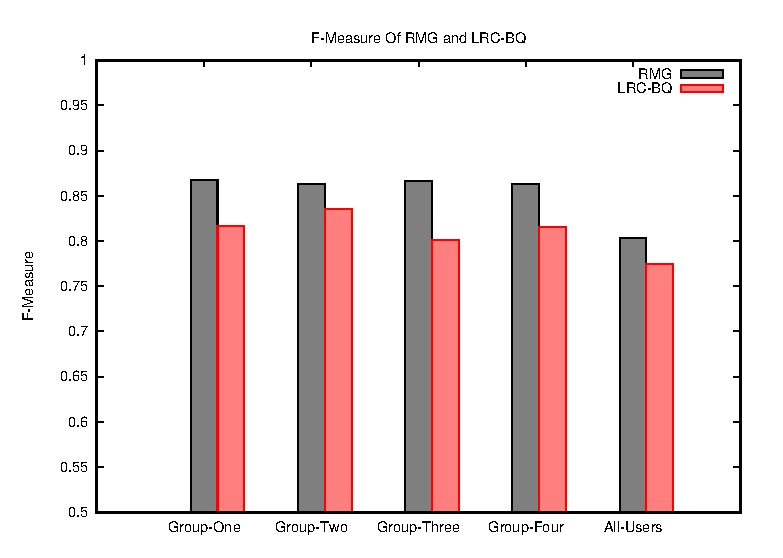
\includegraphics[width=0.32\textwidth]{figures/F-Measure.eps}}
  \caption{Performance of \sys{} Versus LRC-BQ.}
  \label{fig:10}
\end{figure*}


Fig.\ \ref{fig:11} explores the performance of \sys{} when using alternative data items for modeling.
By default, \sys{} uses ``UI+II+MI'', i.e., items of users (UI), microblogs (MI) and interactions (II).
How about using other combinations of the above item(s)?
As shown in Fig.\ \ref{fig:11}, the default setting wins in most cases.

\begin{figure*}
  \centering
  \subfigure[Precision]{
    \label{fig:11-a}
    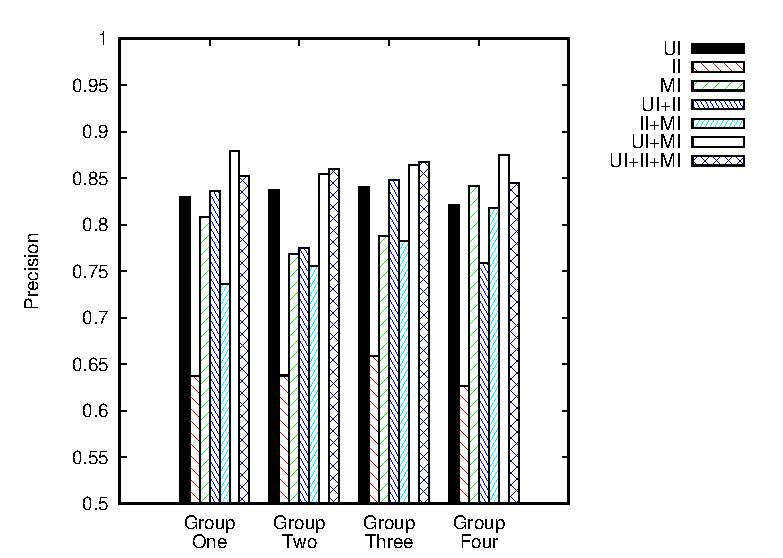
\includegraphics[width=0.32\textwidth]{figures/precisionofdifferentfeatures.eps}}
  %\hspace{1in}
  \subfigure[Recall]{
    \label{fig:11-b}
    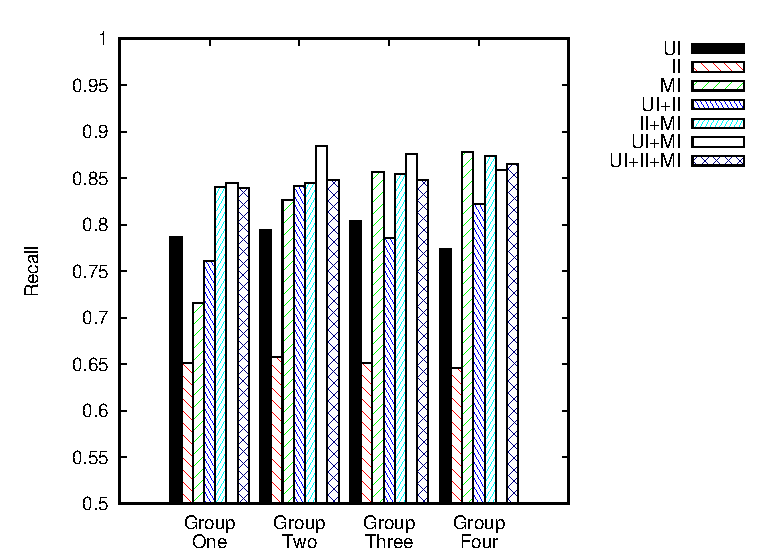
\includegraphics[width=0.32\textwidth]{figures/recallofdifferentfeatures.eps}}
  %\hspace{1in}
  \subfigure[$F_1$ Score]{
    \label{fig:11-c}
    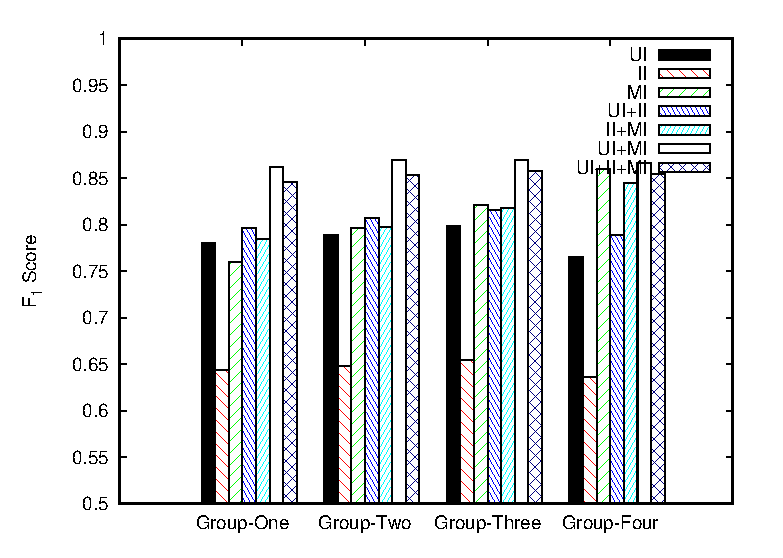
\includegraphics[width=0.32\textwidth]{figures/fmeasureofdifferentfeatures.eps}}
  \caption{\sys{} Performance of Using Various Data Items for Modeling.}
  \label{fig:11}
\end{figure*}

\stitle{Case Study for Feature Extraction}
In this section, we show the results of our demo system for user features extraction.
Considering the huge amount of users, we carefully selected one typical user for analysis.
Here we chose Mary(a famous drama and movie actor in China) as a representative.
The features extraction result for Mary is displayed in Fig.\ \ref{fig:userFeatures}.
Then we can see the basic information of Mary from the result. Her nickname is Actor Mary(��Ա����) and she is from Beijing(����).
The number of followers of Mary is much more than the number of her friends.
The Sina Microblog tag she made for herself is "actor"(��Ա).
As the result of the long-term interest extraction shows, she is interested in stage performances(��̨����), drama performances(�������),films(��Ӱ��Ӱ) and so on, which is consistent with her actual situation.
What's more, the probability distribution of tweeting and retweeting behavior on different time periods in one day indicates that her activities at night is much more than daytime.
The time interval distribution of her behaviors is also shown in Fig.\ \ref{fig:userFeatures}. The time interval is mostly distributed within 48 hours, which indicates that she is a active user.
We developed a function for querying user's short-term interest.
Here we queried Mary's short-term interest between 09/01/2016 and 09/30/2016, and got it as shown in Fig.\ \ref{fig:userFeatures}. We analyzed her microblogs in the this period, she has been working tirelessly to promote the drama "Earl of Oolong Mountain"(����ɽ����). So the results are in line with expectations.

\begin{figure}
  \centering
  \subfigure{
      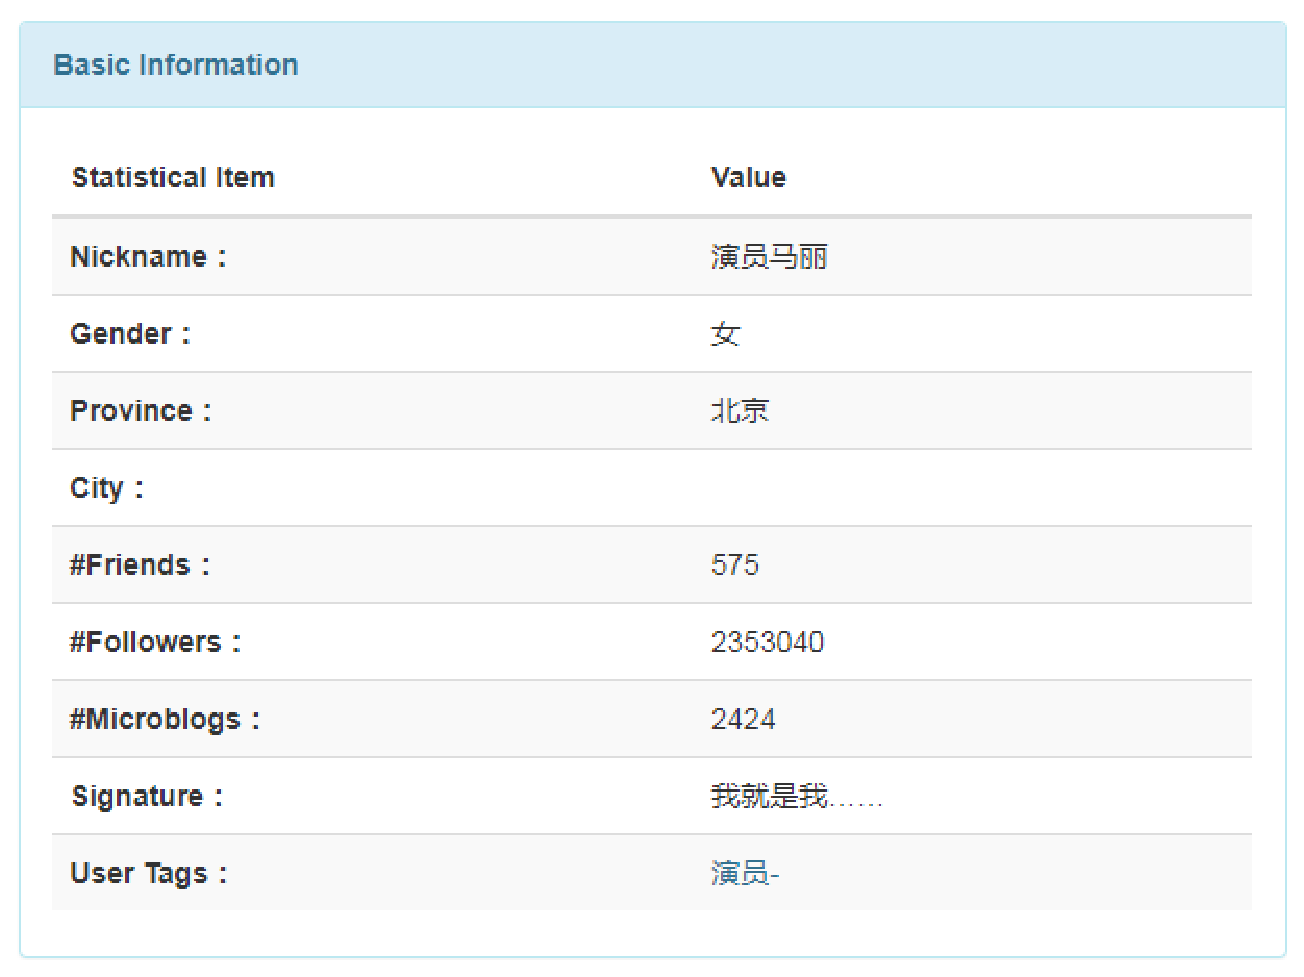
\includegraphics[width=0.22\textwidth]{IMAGE/features/userFeatures/1.eps}}
  \subfigure{
      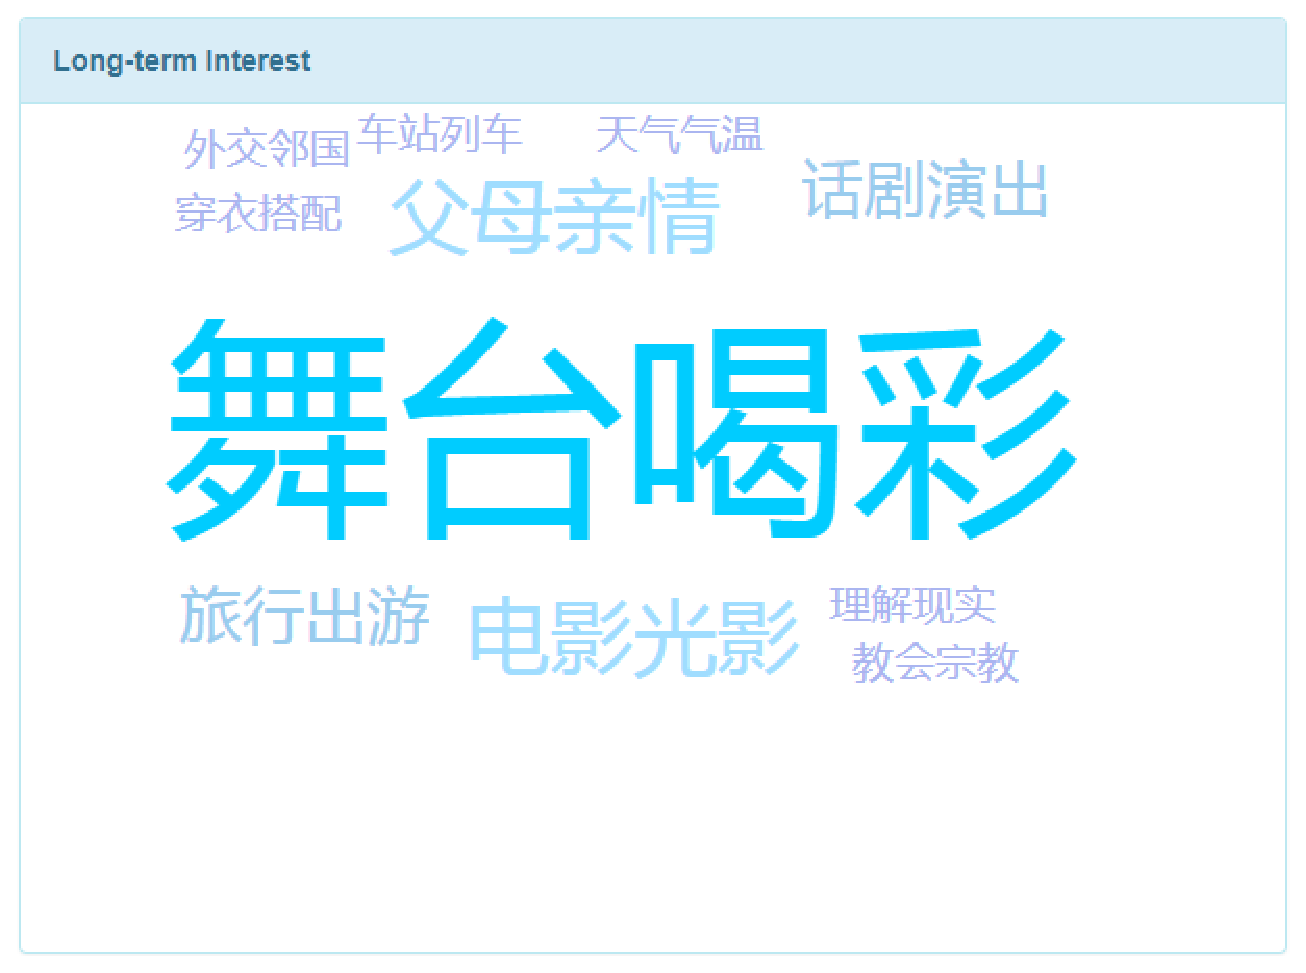
\includegraphics[width=0.22\textwidth]{IMAGE/features/userFeatures/2.eps}}
  \subfigure{
      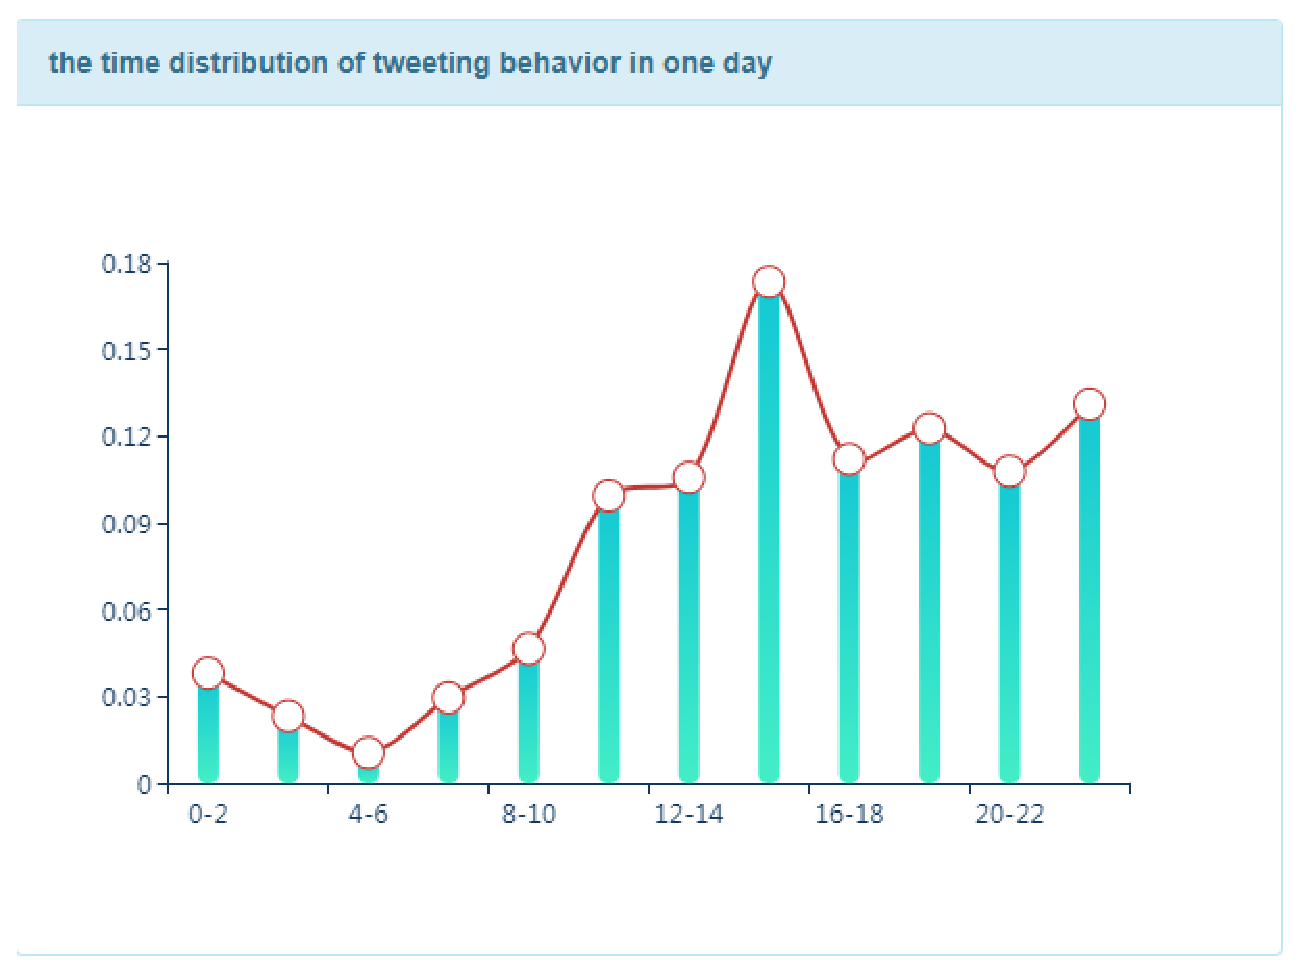
\includegraphics[width=0.22\textwidth]{IMAGE/features/userFeatures/3.eps}}
  \subfigure{
      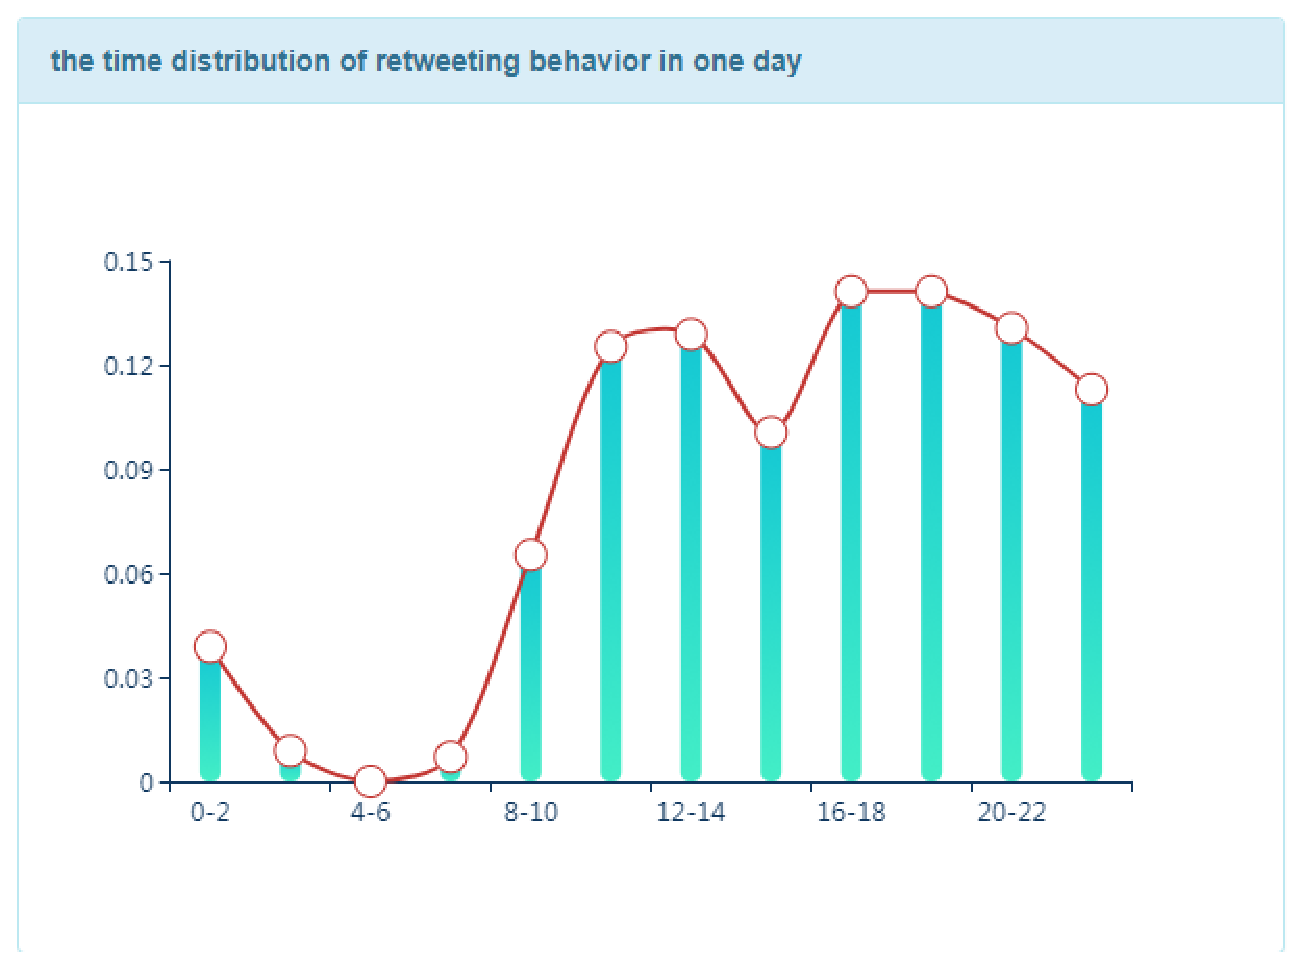
\includegraphics[width=0.22\textwidth]{IMAGE/features/userFeatures/4.eps}}
  \subfigure{
      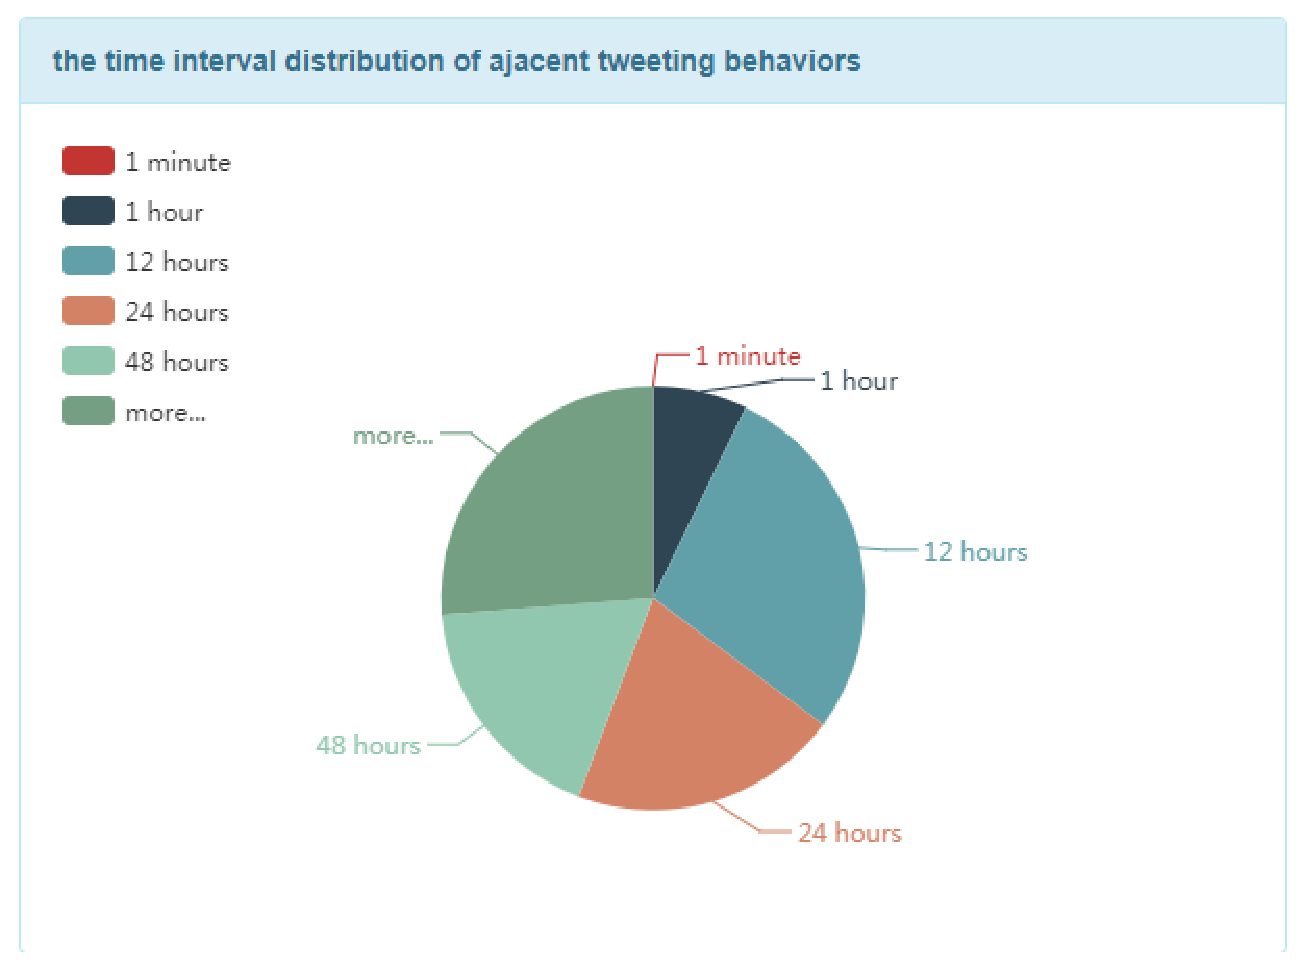
\includegraphics[width=0.22\textwidth]{IMAGE/features/userFeatures/5.eps}}
  \subfigure{
      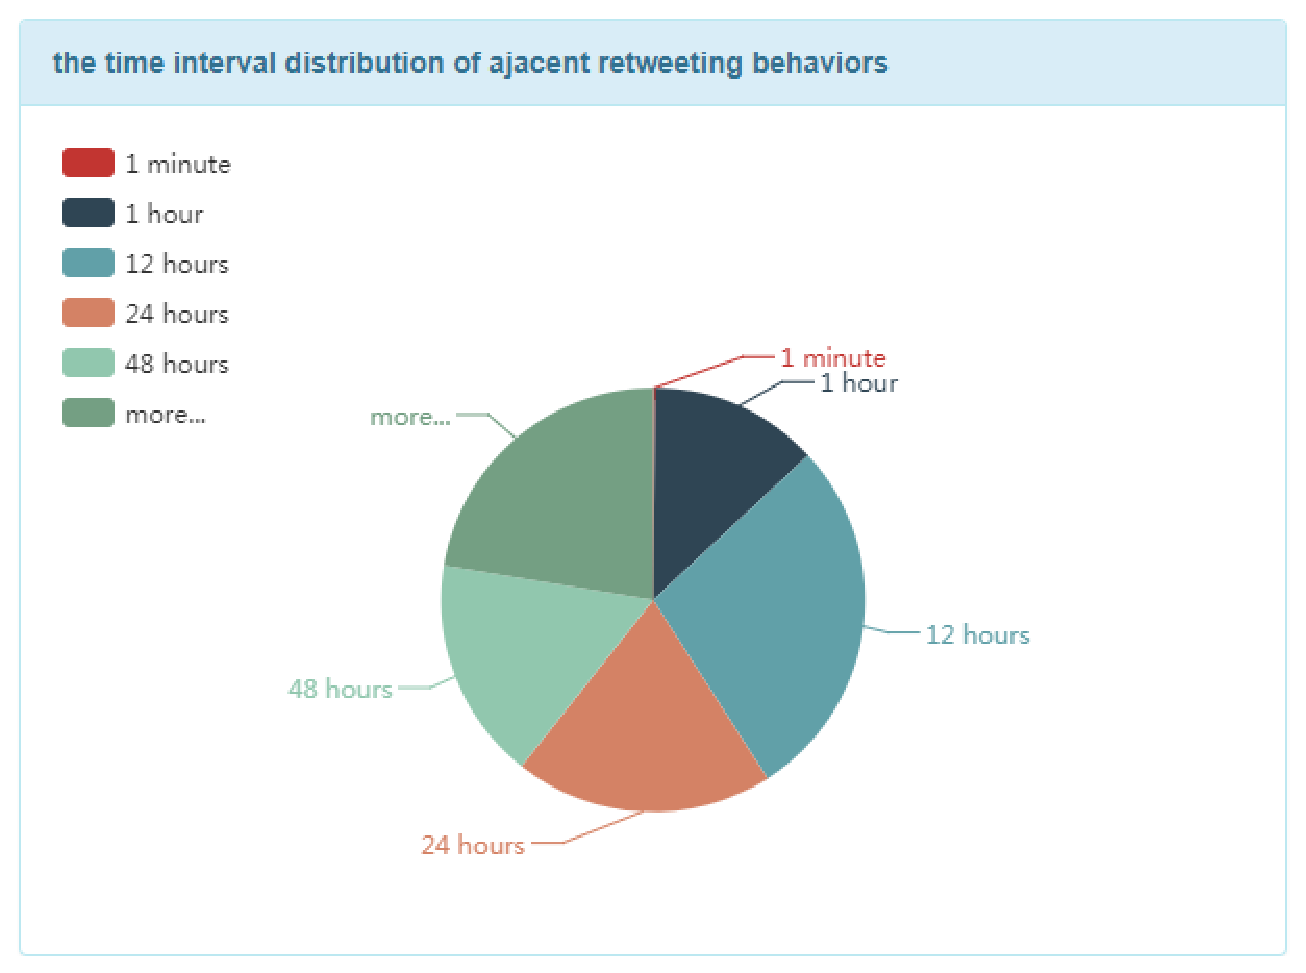
\includegraphics[width=0.22\textwidth]{IMAGE/features/userFeatures/6.eps}}
  \subfigure{
  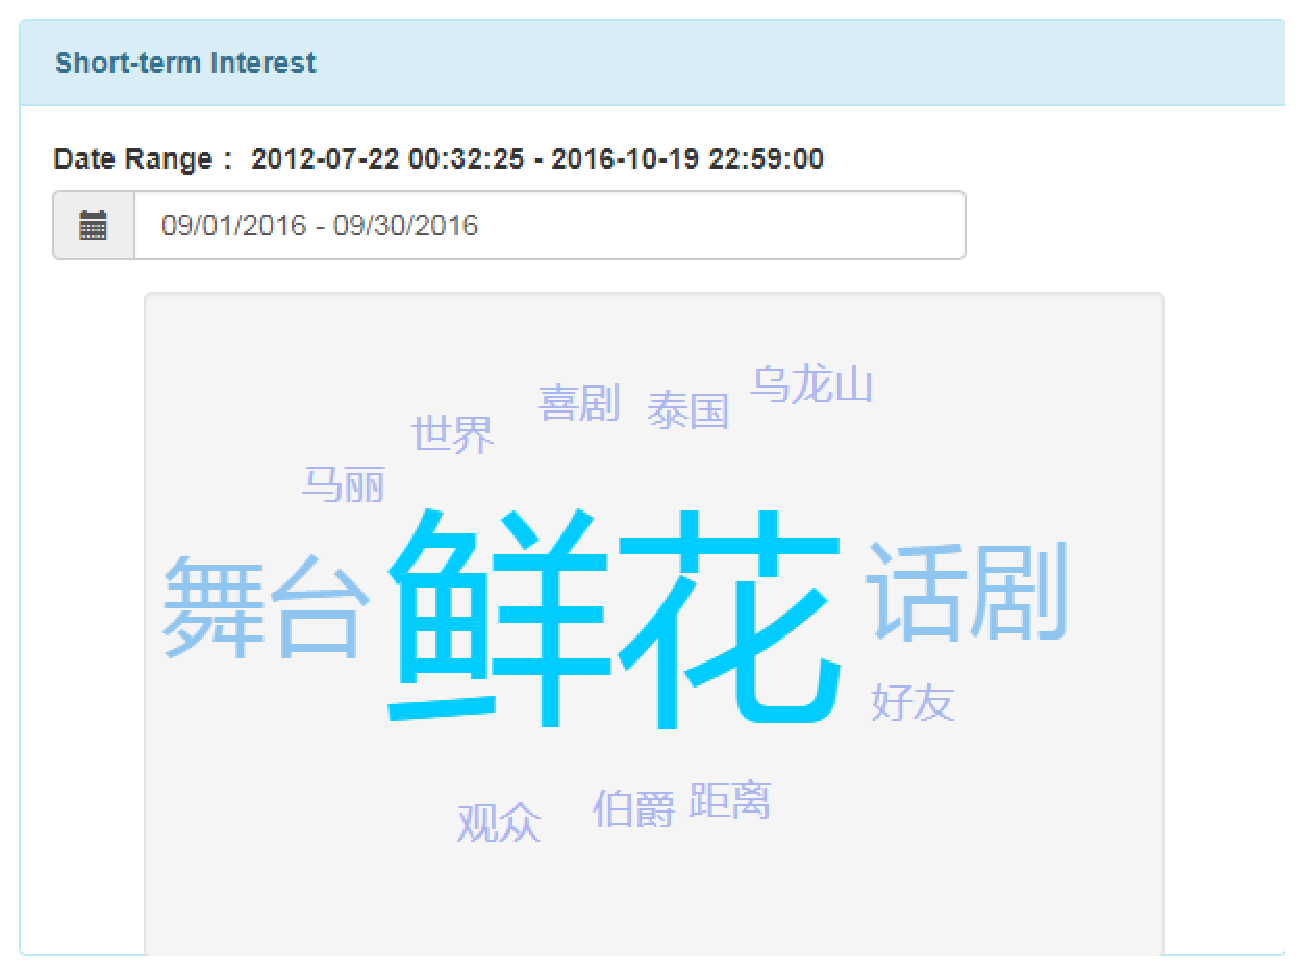
\includegraphics[width=0.22\textwidth]{IMAGE/features/userFeatures/7.eps}}
  \subfigure{
  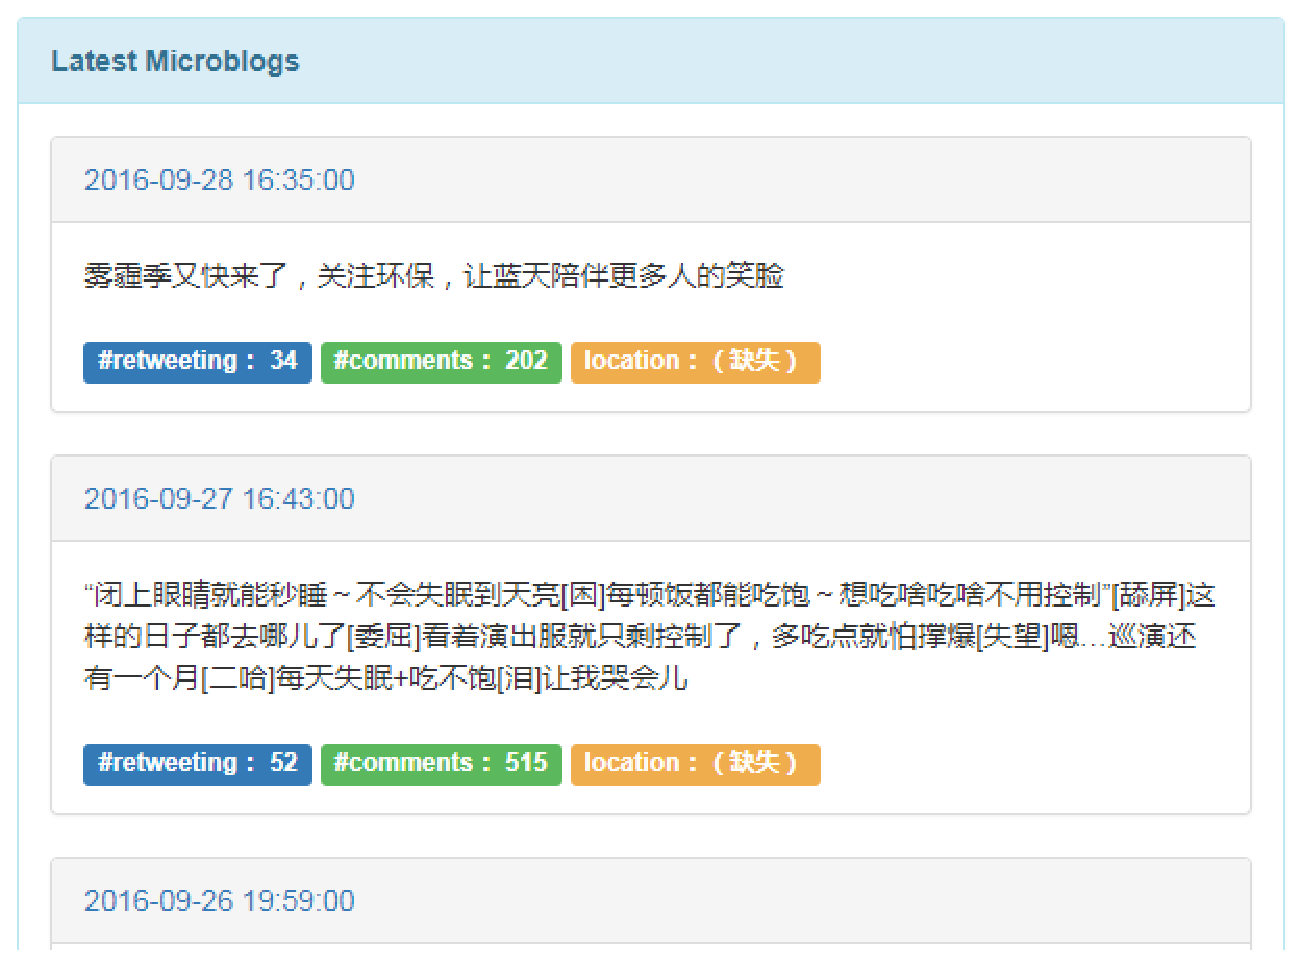
\includegraphics[width=0.22\textwidth]{IMAGE/features/userFeatures/8.eps}}
  \caption{Visualization for User Features.}
  \label{fig:userFeatures} %% label for entire figure
\end{figure}
